\section{Mismatch Cost and Three Regimes}\label{sec:zones}

Consider a decoupled scalar channel with zero signal--noise covariance, correctly specified observation gain and unchanged effective noise. Let signal
variance $p$ and effective noise $q$---sensor noise plus aliased energy---so
that $R=p/(p+q)$. An estimator that assumes variance $\kappa p$ instead of $p$
applies the gain $g=\kappa R/(\kappa R+1-R)$.

\begin{proposition}[Mismatch cost]\label{prop:mismatch}
The excess mean-squared error, normalised by the scalar signal energy $p$, is
\begin{equation}\label{eq:delta}
\Delta(R,\kappa)=\frac{R(1-R)^2(\kappa-1)^2}{(1-R+\kappa R)^2}.
\end{equation}
\end{proposition}
\noindent A proof is in Appendix~\ref{app:proof}. Two limits carry the
prescription:
\begin{itemize}
\item under-estimation, $\kappa\to0$: $\Delta\to R$; harmless when $R$ is low,
costly when $R$ is high;
\item over-estimation, $\kappa\to\infty$: $\Delta\to(1-R)^2/R$; harmless when
$R$ is high, and larger than the band energy itself when $R<0.38$, This compares excess risk to signal energy; total risk exceeds zero reconstruction when $\Delta>R$.
\end{itemize}

\noindent In absolute units, with $Q=\kappa P$ the assumed and $P$ the true
energy and $N$ the effective noise at one frequency,
\begin{equation}\label{eq:delta-abs}
P\,\Delta=\frac{N^2(Q-P)^2}{(P+N)(Q+N)^2}.
\end{equation}
In the well-separated over-estimation limit $P\ll N\ll Q$ the excess error is $\approx N$,
independent of the signal energy; in the well-separated under-estimation limit $Q\ll N\ll P$ it is
$\approx P$. Over-estimation is paid in units of noise, under-estimation in
units of signal \src{DER§1.2}.

\begin{corollary}[Where the asymmetry flips]\label{cor:flip}
In the per-frequency scalar model, for every $\kappa>1$,
$\Delta(R,\kappa)>\Delta(R,1/\kappa)$ if and only if $R<1/2$.
\end{corollary}
\noindent The proof follows from the sign of $(\kappa-1)(1-2R)$
(Appendix~\ref{app:proof}). The statement is exact under two conditions: it is
evaluated per frequency, and the mismatch is a symmetric multiplicative factor
($\kappa$ vs.\ $1/\kappa$). Averaging $R$ and $\kappa$ before applying the nonlinear formula can change the result in either direction; no universal Jensen upper or lower bound applies. Band-level crossover statements are approximate (\S\ref{sec:exp-e2}). The effective noise is held fixed in the scalar model. Random sparse
sampling couples modes, and changing several assumed powers within an
alias set does not preserve a one-channel approximation. This differs from
claiming that physical noise depends on the assumed prior. The sparse
10\% $b_1$ counterexample belongs to this coupled setting.

\paragraph{Three regimes.} We fix two thresholds before the experiments,
$0.8$ and $0.1$ (sensitivity in \S\ref{sec:limits}):
\begin{itemize}
\item \textbf{Regime A} ($\Rlin\ge0.8$): the information is in the
observation. In the limit $R\to1$ over-estimating the spectrum costs
little and under-estimating it costs much, which favours wide, low-bias
representations; the bottleneck is then capacity and optimisation. This is a
per-band tendency, not a rule for choosing a representation: at $R=0.8$ a
$16\times$ over-estimate is not free, and empirical ranking uses the approximate
energy-weighted cost summed over \emph{all} bands, each with its own
$\kappa_b$ (Eq.~\eqref{eq:crit}).
\item \textbf{Regime B} ($0.1\le\Rlin<0.8$): both directions cost; the gain of
spectral adaptation is bounded by
$\mathrm{MSE}_{\rm mismatched}-\mathrm{MSE}_{\rm matched}\ge0$, under that same true-covariance reference; matching can matter, but closeness to an oracle does not establish practical selection.
\item \textbf{Regime C} ($\Rlin<0.1$): the chosen stationary reference has low expected recovery. Strong under-estimation incurs at most $R$ excess; arbitrary over-estimation need not be safe. Alternative structured priors, including nonstationary linear models or learned nonlinear models, may recover more on real signals. This reference regime is not an impossibility theorem.
\end{itemize}

\paragraph{Zone labels do not pick winners.} To compare representations with
effective priors $Q$ we use the band-summed, absolute cost
\begin{equation}\label{eq:crit}
C(Q)=\sum_b E_b\,\Delta\big(R_b,\kappa_b(Q)\big),
\end{equation}
with band energy $E_b$, matched-prior recoverability $R_b$ and
$\kappa_b(Q)$ the ratio of candidate to reference prior-spectrum band integrals; lower $C$
is predicted better. In D11, the spectrum ratio is on the 512 grid, while $E_b$ is truth energy after HR240 cropping and a Hann window. Their numerical definitions differ; the substitution is a diagnostic approximation. For linear arms the exact trace formula
$\mathbb{E}\|x-\hat x\|^2=\operatorname{tr}\!\big((I-H_QA)C_P(I-H_QA)^\top\big)+\sigma_n^2\|H_Q\|_F^2$
needs no approximation. Eq.~\eqref{eq:crit} ranks representations
(E2: 0.90; D11: 0.856) but does not reliably select the best among close
candidates (D11: 1/3), does not cover non-linear iterative fits, and its
a-priori version (generic spectrum for $E_b$, $\kappa_b$) has not been tested
(\S\ref{sec:exp-ab}) \src{DER§2.3}. The per-frequency scalar form
Eq.~\eqref{eq:delta-abs} illustrates why over-estimation is paid in units of
noise but is not used as evidence: for non-diagonal operators (random shifts,
sparse sampling) its per-frequency predictions are inaccurate.

\paragraph{Qualitative interpretations to test.}
(i) Grid or hash fields without spectral decay can express high frequencies with weak regularisation; they can deteriorate under noise, but no equivalent fixed prior $Q$ has been identified here;
(ii) Fourier features with large $\sigma$ in SuperF-style fitting can show similar empirical deterioration;
(iii) a regulariser of fixed strength corresponds to a fixed $\kappa$ relative
to a noise-dependent $p/q$, so its effective mismatch drifts with noise.
\S\ref{sec:exp-ab} tests these on multi-frame SR.

\begin{table*}[t]\centering\small
\caption{A-priori three-regime map: $\Rlin$ per band under the generic
$1/f^2$ prior, no data, no training \src{OUT3/d8}.
Shading: A $\ge0.8$, B, C $<0.1$.}\label{tab:map}
\begin{adjustbox}{max width=\linewidth}\begin{tabular}{llccc}\toprule
Task & $\sigma_n$ & $b_1$ & $b_2$ & $b_3$\\\midrule
Single image $\times2$ & .002 / .01 & 1.00 / 1.00 & .92 / .90 & .09 / .08\\
Single image $\times4$ & .002 / .01 & .98 / .98 & .09 / .08 & .01 / .01\\
Single image $\times8$ & .002 / .01 & .79 / .77 & .01 / .01 & .01 / .01\\
Sparse 5\% & .002 & .70 & .09 & .03\\
Sparse 10\% & .002 & .81 & .20 & .07\\
Sparse 25\% & .002 & .92 & .47 & .20\\
Sparse 50\% & .002 & .98 & .76 & .46\\
Multi-frame $\times4$, $T{=}4$ & .002$\to$.02 & $\approx$1.0 & .73$\to$.51 & .12$\to$.03\\
Multi-frame $\times4$, $T{=}8$ & .002$\to$.02 & $\approx$1.0 & .83$\to$.62 & .27$\to$.08\\
Multi-frame $\times4$, $T{=}16$ & .002$\to$.02 & $\approx$1.0 & .90$\to$.73 & .41$\to$.15\\
\bottomrule\end{tabular}\end{adjustbox}
\end{table*}

\begin{figure*}[t]\centering
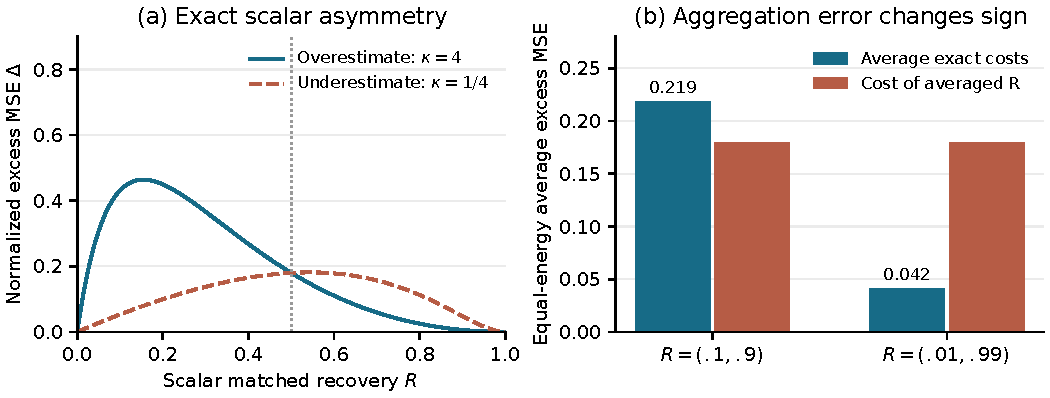
\includegraphics[width=.95\textwidth]{figures/scalar-cost.pdf}
\caption{Exact scalar mismatch and limits of band averaging. (a) Reciprocal
mismatches cross at $R=.5$ under fixed effective noise. (b) Equal-energy
modes with the same average $R=.5$ and $\kappa=4$ produce aggregation errors
of opposite sign. This analytic figure does not imply scalar decoupling
for the experimental observation operators.}\label{fig:cost}
\end{figure*}

\paragraph{Two ways to assign a regime.}
$\Rlin$ describes what the observation permits a linear estimator; it is the
right axis for linear, multi-frame, sparse and 1D tasks, and it is computable
in advance. A trained ASISR network, however, lifts regime-C bands to
intermediate recovery through its learned prior (\S\ref{sec:exp-c}). To
describe what components \emph{inside} such a network do, the regime has to
be assigned by the network's actual recovery $\Rnet$, which requires ground
truth and is therefore a post-hoc description, not a prediction
(\S\ref{sec:exp-f1}).
At this network layer Prop.~\ref{prop:mismatch} is not a theorem: a
network is not a fixed linear Wiener estimator with a known $\kappa$.
Nor do $\Rnet\approx0$ or $1$ force small ablation loss: removing a component
can worsen a perfectly recovered band, or improve a poorly recovered one.
The measured concentration of losses is therefore empirical, not a
necessary boundary condition. No scalar asymmetry or causal mechanism is
inferred from these network measurements.
